\chapter{I'm A Chapter}

\section{I'm a Section}

\subsection{I'm a Subsection}

I'm Text. (Hi!)  I'm here to demonstrate that this class will automatically take care of proper paragraph indentation, line spacing and pagination.

\section{I'm A New Section}

\subsection*{I'm an Unnumbered Subsection}

\begin{equation}
E = mc^2 \alpha \gamma \Gamma
\end{equation}

The coefficient of lift, $C_{Lift_0}$

\subsection*{I'm an Unnumbered Subsection that will nevertheless appear in the Table of Contents}
\addcontentsline{toc}{subsection}{I'm an Unnumbered Subsection that will nevertheless appear in the Table of Contents}

I'm more text.  I'm text that refers to Figure \ref{fig:sample_figure}.  I'm text that refers to Table \ref{tbl:sample_table}.

\begin{figure}[ht]
\centering
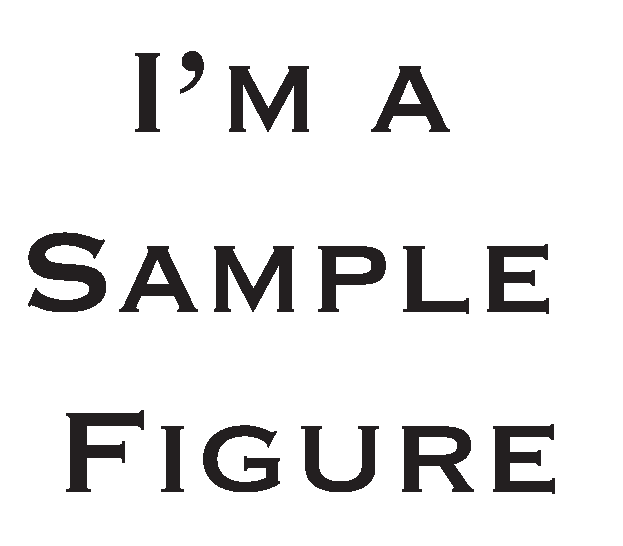
\includegraphics[width=0.5\textwidth]{sample_figure}
 \caption[Sample Caption]{ I'm a sample figure caption.\label{fig:sample_figure} }
\end{figure} 

Paragraph of text about figures...

\begin{figure}[Ht]
\centering
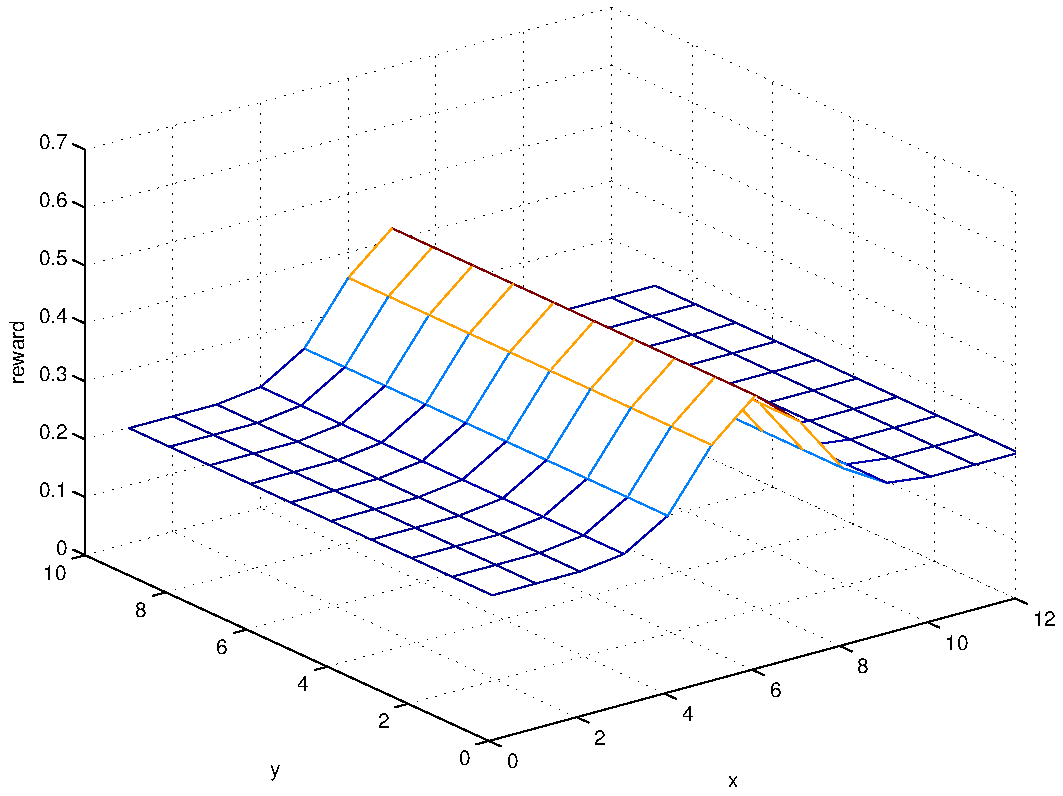
\includegraphics[width=0.75\textwidth]{cgRewardGrid.pdf}
 \caption[Sample Caption]{ I'm a sample figure caption.\label{fig:sample_figure} }
\end{figure} 


\begin{table}[ht]
\centering
\caption[Sample Table]{I'm a sample table caption.}\label{tbl:sample_table}
\vspace{.1in}
\begin{tabular}{| c | l  l  l |}
\hline\hline
Column 1 &  Column 2 & Column 3 & Column 4\\
\hline
0 & 1& 2& 3\\
4 & 5& 6 & 7\\
\hline
\end{tabular}
\end{table}
